\begin{quote}
The aim of the Peeragogy Handbook is to lay out effective peer-learning
techniques that you can implement ``on the ground.'' We suggest that you
look through the Handbook, try a few of these suggestions, and see how
they work for you. Then we invite you to return here, share your
experiences, ask for feedback, and work with us to improve the Handbook
and the field we affectionately call ``Peeragogy.''

In this part of the Peeragogy Handbook, teams of ``peeragogues'' have
distilled their most important and applicable research and insights from
more than a year of inquiry and discussion. Although there's been no
shortage of experimentation and formal research into collaborative,
connective, and shared learning systems in the past, we've detected a
new rumbling among education thinkers that when combined with new
platforms and technologies, peer-learning strategies as described here
could have a huge impact on the way educational institutions evolve in
the future. We've also seen for ourselves how peer learning techniques
can help anyone who's interested become an effective informal educator,
whether or not that's part of their job description.
\end{quote}

\begin{figure}[htbp]
\centering

\includegraphics[width=.4\textwidth]{../pictures/peeragogy-in-action.jpg}
\end{figure}

\subsection{The interplay of individual and group}

``Personal'' supports ``peer'' - We can consciously cultivate living,
growing, responsive webs of information, support, and inspiration that
help us be more effective learners. This is a personal learning network.
We'll offer tips on how to build these networks --- and we'll also
explain how strong personal learning networks can contribute to and
evolve into even stronger peer learning networks.

``Peer'' supports ``personal'' - As we work together to develop shared
plans for our collective efforts in group projects, we usually can find
places where we have something to learn. Furthermore, if we are willing
to ask for help and offer our help to others, everybody's learning
escalates. Being mindful of effective interpersonal learning patterns is
an important part of building an effective personal learning plan.

In the following sections, you can read some more about these
strategies, or you can skip ahead to Part III to start looking at
specific techniques you can use to build your own peer learning group.

\subsection{Peer learning through the ages}

As you may have guessed, our new term, peeragogy, is a riff on the word
pedagogy --- the art, science, or profession of teaching. Pedagogy has a
somewhat problematic story of origin: it comes from the ancient Greek
tradition of having a child (paidos) be supervised (agogos) by a slave.
Greek philosophers disagreed with each other as to the best way for
individuals to gain knowledge (and even more so, wisdom). Socrates, who
insisted that he was not wise, also insisted that his interlocutors join
him in investigating truth claims, as peers. The most famous of these
interlocutors, Plato, on a more pedagogical bent, spoke of an
enlightened few, whose responsibility it was to show others the light of
knowledge (illustrated by his famous allegory of ``The Cave'').

In more recent centuries, various education theorists and reformers have
challenged the effectiveness of what had become the traditional
teacher-led model. Most famous of the early education reformers in the
United States was John Dewey, who advocated new experiential learning
techniques. In his 1916 book, Democracy and Education {[}1{]}, Dewey
wrote, ``Education is not an affair of `telling' and being told, but an
active and constructive process.'' Soviet psychologist Lev Vygotsky, who
developed the concept of the Zone of Proximal Development, was another
proponent of ``constructivist'' learning. His book, Thought and
Language, also gives evidence to support collaborative, socially
meaningful, problem-solving activities over solo exercises.

Within the last few decades, things have begun to change very rapidly.
In Connectivism: A Learning Theory for the Digital Age, George Siemens
argues that technology has changed the way we learn, explaining how it
tends to complicate or expose the limitations of the learning theories
of the past {[}3{]}. The crucial point of connectivism is that the
connections that make it possible for us to learn in the future are more
relevant than the sets of knowledge we know individually, in the
present. Furthermore, technology can to some degree and in certain
contexts, replace know-how with know-where-to-look.

If you want more details on the history, theories, and recent
experiments related to peer learning, we have a more extensive
literature review available. We've also adapted it into a Wikipedia
page, which you can edit as well as read.

\begin{figure}
\begin{center}
\href{http://commons.wikimedia.org/wiki/File:Platon\_Cave\_Sanraedam\_1604.jpg}{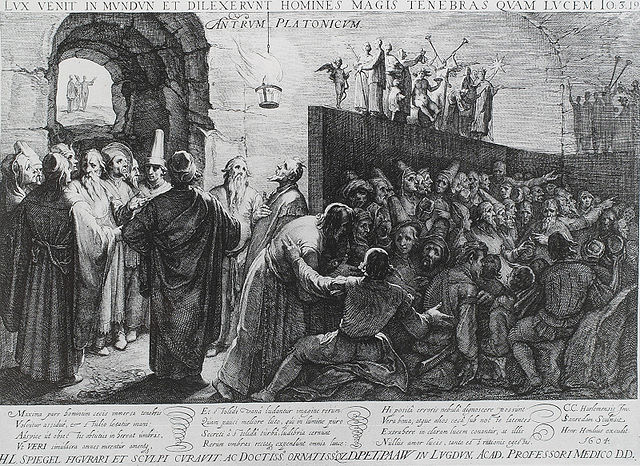
\includegraphics[width=.8\textwidth]{../pictures/plato_cave.jpg}}
\end{center}
\caption*{\href{http://commons.wikimedia.org/w/index.php?title=File:Platon\_Cave\_Sanraedam\_1604.jpg\&oldid=68567627}{Platon Cave Sanraedam (1604)}. By Jan Saenredam {[}Public domain{]}, via
Wikimedia Commons}
\end{figure}

\subsection{From peer learning to peeragogy}

The idea that we needed a new theory (which we gave the name
\emph{paragogy} {[}4{]}) arose out of the challenges we faced doing peer
learning. Our aim was to understand how groups and organizations can get
better at serving participants' interests, while participants also learn
and becoming better contributors.

Paragogy started out as a set of proposed principles that describe peer
produced peer learning -- we'll say exactly what these principles are a
bit further below. We designed them to contrast with a set guidelines
for adult educators advanced by Malcolm Knowles {[}5{]}. The paragogy
principles focused on the way in which co-learners shape their learning
context together. Peer produced peer learning is something for
``innovative educators'' everywhere, working at all scales. You don't
need to have the word teacher, trainer, or educator in your job title.
It's enough to invite someone out to lunch and ask questions, set up a
reading group with your friends, or even to tackle a new DIY project
following tips from the hardware store clerk or instructions you
downloaded from the internet.

Our secret for successful peer learning is actually hidden in plain
view: the word ``paragogy'' means ``production'' in Greek. We're
particularly interested in how the powerful blend of peer learning and
collaborative work drives open source software development, and helps
build resources like Wikipedia. But in fact it works equally well in
offline settings, from official hacker/maker spaces to garages and
treehouses. Projects like
\href{http://storycorps.org/about/}{StoryCorps} show how contemporary
media can add a powerful new layer to ancient strategies for teaching,
learning, and sharing.

The word ``peeragogy'' attempts to make these ideas immediately
understandable to everyone, including non-geeks. Peeragogy is about
peers learning together, and teaching each other. In the end, the two
words are actually synonyms. If you want to go into theory-building
mode, you can spell it ``paragogy''. If you want to be a bit more down
to earth, stick with ``peeragogy.''

\subsection{References}

\begin{enumerate}
\item
  Dewey, J. (2004). Democracy and education. Dover Publications.
\item
  Vygotsky, L. S. (1986). Thought and language. MIT press.
\item
  Siemens, G. (2005). Connectivism: A learning theory for the digital
  age. International Journal of Instructional Technology and Distance
  Learning, 2(1), 3-10.
\item
  Corneli, J. and Danoff, C.J. (2011), Paragogy: Synergizing individual
  and organizational learning. (Published on Wikiversity.)
\item
  Knowles, M. S. (1980). The modern practice of adult education: From
  pedagogy to andragogy. Chicago: Follett.
\end{enumerate}
